\documentclass{article}

\usepackage{url}
\usepackage{amsmath,amssymb}
\usepackage{graphicx,svg}

\begin{document}
\title{Lecture 10\\ Inverse Laplace Transform}
\author{C.L. Wyatt}
\date{\today}
\maketitle

In today's lecture we introduce the Inverse Laplace Transform for CT signals and systems.

\section{Inverse Unilateral Laplace Transform}

Consider a causal function $f(t)$ that may or may not be absolutely integrable. Let $g(t)=f(t) e^{-c t}$ for some $c>0$ such that

$$
\int_{0}^{\infty}|g(t)| dt = \int_{0}^{\infty}\left|f(t) e^{-c t}\right| dt < \infty
$$

Then the Fourier Transform of $g(t)$ exists

$$
\begin{aligned}
G(\omega) & =\int_{-\infty}^{\infty} g(t) e^{-j \omega t} dt = \int_{0}^{\infty} f(t) e^{-c t} e^{-j \omega t} dt \\
& =\int_{0}^{\infty} f(t) e^{-(c+j \omega) t} dt \\
& =\left.\mathcal{L}_{1}\{f(t)\}\right|_{s = c+j\omega} \quad c \text{ fixed s.t. } c+j\omega \in \text{ROC}
\end{aligned}
$$

The inverse Fourier Transform is

$$
g(t)=f(t) e^{-c t}=\frac{1}{2 \pi} \int_{-\infty}^{\infty} G(\omega) e^{j \omega t} d\omega
$$

multiply through by $e^{c t}$

$$
\begin{aligned}
e^{c t} g(t)=f(t) & =\frac{1}{2 \pi} \int_{-\infty}^{\infty} G(\omega) e^{c t} e^{j \omega t} d\omega \\
& =\frac{1}{2 \pi} \int_{-\infty}^{\infty} G(\omega) e^{(c+j \omega) t} d\omega
\end{aligned}
$$

Substitute $G(\omega)$\\
$$
f(t)=\frac{1}{2 \pi} \int_{-\infty}^{\infty}\left[\underbrace{\int_{0}^{\infty} f(\tau) e^{-(c+j \omega) \tau}}_{\left.F(s)\right|_{s=c+j \omega}} d\tau\right] e^{(c+j \omega) t} d \omega
$$
$$
f(t)=\frac{1}{2 \pi} \int_{-\infty}^{\infty} F(c+j \omega) e^{(c+j \omega) t} d \omega
$$

Let $s=c+j \omega$. Since $c$ is a constant $ds = 0+j d\omega$ implying $d \omega=\frac{1}{j} d s$
and
$$
f(t)=\frac{1}{2 \pi j} \int\limits_{c-j\infty}^{c+j\infty} F(s) e^{st}\; ds
$$
a complex integral.

Note: we can think of $c$ as the real values such that $f(t) e^{-c t}$ has a Fourier Transform. This is the ROC.

Does the above integral look like our contar Integrals from previous lectures?

Yes, if we use the Bromwitch contour.

\begin{figure}
  \centering
  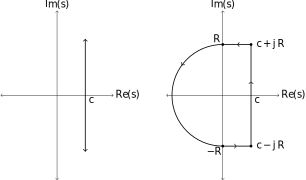
\includegraphics[alt={contour of integration for inverse laplace transform. See caption.}]{figures/fig10_1.svg}
  \caption{The linear contour of integration for the inverse Laplace transform becomes the Bromwitch contour as $R\rightarrow\infty$.}
\end{figure}

$$
f(t)=\frac{1}{2 \pi j} \int\limits_{c-j \infty}^{c+j \infty} F(s) e^{s t} d s = \lim_{R \rightarrow \infty} \oint_{C(R)} F(s) e^{s t} ds
$$

where $C(R)$ is the Bromwitch contour.\\


This allows us to use the method of residues since $C \in \text{ROC}$ implies $C(R)$ encloses all singulartes of $F(s)$.

\textbf{Example:} Recall that $\mathcal{L}\{x(t)\}=\mathcal{L}\left\{e^{-a t} u(t)\right\}$ for $a\in \mathbb{R}$ was $\frac{1}{s+a} \text{Re}(s) > -a$

Then

$$
x(t)=\mathcal{L}_1 \left\{\frac{1}{s+a}\right\}=\frac{1}{2 \pi j} \int_{c-j \infty}^{c+ j\infty} \frac{1}{s+a} e^{s t} d s \quad \text{for} c > -a
$$
or using the Bromwitch contour
$$
x(t) =\lim_{R \rightarrow \infty} \frac{1}{2 \pi j} \oint_{C(R)} \frac{e^{s t}}{s+a} ds  \qquad c>-a
$$

Now from last time, since $e^{s t}$ is analytic and $C(R)$ encloses the singulary at $-a$, from the Residue Theorem

$$
\oint \frac{e^{st}}{s+a}\; ds = 2\pi j k_1
$$
where the residual is

$$
k_1 = \left. (s+a) \frac{e^{st}}{s+a} \right|_{s = -a} = \left. e^{st} \right|_{s = -a} = e^{-a t} \qquad t > 0  
$$

Thus

$$
x(t) = \frac{1}{2\pi j} \cdot 2\pi j e^{-at} \qquad t > 0 = e^{-at}u(t)
$$

\section{Inverse Bilateral Laplace Transform}

Given a non-causal signal $x(t)$ we can write it as

$$
x(t) =\underbrace{x_{1}(t) u(-t)}_{\text{anticausal part}} +\underbrace{x_{2}(t) u(t)}_{\text{causal part}}
$$
    
$$
\begin{aligned}
  L_2\left\{ x(t) \right\} &= \int_{-\infty}^{0} x_{1}(t) e^{-s t} \; dt + \int_{0}^{\infty} x_{2}(t) e^{-s t} \; dt\\
  &= \int_{0}^{\infty} x_{1}(-t) e^{s t} \; dt + \mathcal{L}_1 \left\{x_{2}(t)\right\}\\
  &= \left. \mathcal{L}_1 \left\{x_{1}(-t)\right\} \right|_{s = -s} + \mathcal{L}_1 \left\{x_{2}(t)\right\}\\
  X(s) &= \underbrace{X_1(s)}_{\text{Re}(s) < U} + \underbrace{X_2(s)}_{\text{Re}(s) > L}
\end{aligned}
$$
where the ROC of $X(s)$ is the intersection of the ROC for $X_1$ and $X_2$, a strip in the complex plane $L < \text{Re}(s) < U$.

To use this for the inverse we apply this in reverse.

$$
x(t) = \left. \mathcal{L}_1^{-1}\left\{X_1(-s)\right\}\right|_{t\rightarrow -t} +  \mathcal{L}_1^{-1}\left\{X_2(s)\right\}
$$


\textbf{Example:} Recall an example of a forward bilateral Laplace transform from lecture 9
$$
\mathcal{L}_{2}\left\{e^{-|t|}\right\}=\underbrace{\frac{-1}{s-1}}_{\text{Re}(s) < 1}+\underbrace{\frac{1}{s+1}}_{\text{Re}(s) > -1} = X(s)
$$

Then
$$
x(t)=\mathcal{L}_{2}^{-1}\{X(s)\}=\left.\mathcal{L}_{1}^{-1}\left\{\frac{1}{s+1}\right\}\right|_{t\rightarrow -t} \mathcal{L}_1^{-1}\left\{\frac{1}{s+1}\right\}
$$

From our previous result when $a=1$

$$
\begin{aligned}
x(t) & =\left.e^{-t} u(t)\right|_{t \rightarrow -t}+e^{-t} u(t) \\
& =e^{t} u(-t)+e^{-t} u(t)=e^{-|t|} 
\end{aligned}
$$

\textbf{Example:} Find the inverse Laplace transform of
$$
X(s) = \frac{1}{s} \quad \text{Re}(s) > 0\; .
$$

Solution: Since the ROC corresponds to a causal signal, for $t > 0$
$$
\begin{aligned}
x(t) &= \frac{1}{2 \pi j} \int\limits_{c-j \infty}^{c+j \infty} X(s) e^{s t} \; ds \quad c > 0 \\
  &= \frac{1}{2 \pi j} \oint \frac{e^{s t}}{s} \; ds\\
&= \frac{1}{2 \pi j} 2 \pi j \; k \\
&= \left.s \frac{e^{st}}{s}\right|_{s=0}\\
&=1 \quad t > 0 \\
\end{aligned}
$$
which can be written as $x(t) = u(t)$ for all times $t$.

\textbf{Example:} Find the inverse Laplace transform of
$$
X(s) = \frac{10}{s^{2} + 5s + 6} \quad \text{Re}(s) >-2 \; .
$$

First we use the partial fraction expansion.

\[
X(s) = \frac{10}{(s+2)(s+3)} =\frac{A}{s+2}+\frac{B}{s+3}
\]

\[
A=\left.\frac{10}{s+3}\right|_{s=-2}=\frac{10}{1}=10
\]

\[
B=\left.\frac{10}{s+2}\right|_{s=-3}=\frac{10}{-1}=-10
\]


Then
\[
x(t)=\mathcal{L}_{1}^{-1}\left\{\frac{10}{s+2}\right\}+\mathcal{L}_{1}^{-1}\left\{\frac{-10}{s+3}\right\}
\]

Using the Residue theorem,

$$
\begin{aligned}
x(t)&=\frac{10}{2 \pi j} \int\limits_{c-j\infty}^{c+j \infty} \frac{e^{s t}}{s+2} \; ds - \frac{10}{2 \pi j} \int\limits_{c-j \infty}^{c+j \infty} \frac{e^{s t}}{s+3} \; ds \\
& c>-2 \quad c>-2 \\
& =\frac{10}{2 \pi j} \oint \frac{e^{s t}}{s+2} \; d s - \frac{10}{2 \pi j} \oint \frac{e^{s t}}{s+3} \; ds \\
& =\frac{10}{2 \pi j} 2 \pi j e^{-2 t} - \frac{10}{2 \pi j} 2 \pi j e^{-3 t} \\
&=10 e^{-2 t}-10 e^{-3 t} \quad t>0
\end{aligned}
$$

Writing the expression for all $t$ gives:

\[
x(t)=10\left(e^{-2 t}-e^{-3 t}\right) u(t) .
\]

\textbf{Example:} Here is an example with complex singularties. Find the inverse Laplace transform of

$$
X(s)=\frac{s}{s^{2}+2 s+5} \quad \text{Re}(s)>-1
$$

Using the partial fraction expansion

\[
X(s) = \frac{s}{(s + 1 + j2)(s + 1 - j2)} = \frac{A}{s + 1 + j2} + \frac{B}{s + 1 - j2} 
\]
where
\[
A=\frac{-1-j2}{-1-j2+1-j2}=\frac{-1-j2}{-j4}=\frac{1}{2}-\frac{1}{4} j
\]

\[
B=\frac{-1+j2}{-1+j2+1+j2}=\frac{-1+j2}{j4}=\frac{1}{2}+\frac{1}{4} j
\]


Then

\[
x(t) = \mathcal{L}_{1}^{-1}\left\{\frac{\frac{1}{2}-\frac{1}{4} j}{s+1+j2}\right\}+\mathcal{L}_{1}^{-1}\left\{\frac{\frac{1}{2}+\frac{1}{4} j}{s+1-j2}\right\}
\]

Using residues, let $c = 0 > -1$

$$
x(t) = \frac{1}{2 \pi j} \int\limits_{-j \infty}^{j\infty} \frac{\frac{1}{2}-\frac{1}{4} j}{s+1+j2} e^{st}\; ds + \frac{1}{2 \pi j} \int\limits_{-j \infty}^{j\infty} \frac{\frac{1}{2}+\frac{1}{4} j}{s+1-j2} e^{st}\; ds 
$$

\[
x(t)=\frac{1}{2 \pi j} 2 \pi j \, k_{1}+\frac{1}{2 \pi j} 2 \pi j\, k_{2}
\]

$$
\begin{aligned}
& k_{1}=\left(\frac{1}{2}-\frac{1}{4} j\right) e^{(-1-j 2) t} \quad k_{2}=\left(\frac{1}{2}+\frac{1}{4} j\right) e^{(-1+j 2) t} \\
& x(t)=k_{1}+k_{2}=\left(\frac{1}{2}-\frac{1}{4} j\right) e^{(-1-j 2) t}+\left(\frac{1}{2}+\frac{1}{4} j\right) e^{(-1+j 2) t} \\
& \text { } \quad \text{for } t > 0 
\end{aligned}
$$

with some effort you can write this as

$$
x(t)=e^{-t}\left(\cos (2 t)-\frac{1}{2} \sin (2 t)\right)\; u(t)
$$

for all $t$.

\end{document}
